% Plantilla común para figuras redibujadas (fig-NN-desc.tex).
% Copiar entera y sustituir solo el cuerpo entre las marcas "cuerpo de la figura".
% Compila tal cual en Overleaf o con scripts/tikz2svg.sh.
%
% NO añadir la opción "tikz" a standalone: parte cada tikzpicture (y cada
% \chemfig) en una página distinta y el SVG solo tendría la primera.
\documentclass[border=4pt]{standalone}
\usepackage[T1]{fontenc}
\usepackage{lmodern}            % base vectorial: sin fuente vectorial el texto sale en Type 3 y dvisvgm lo pierde
\usepackage[scaled=0.95]{helvet}% sans-serif tipo Helvetica, como la interfaz de Obsidian
\renewcommand{\familydefault}{\sfdefault}
\usepackage{amsmath,amssymb}
\usepackage{sansmath}\sansmath  % fórmulas en sans, a juego con el texto
\usepackage[version=4]{mhchem}  % \ce{A + B -> C}
\usepackage{chemfig}            % estructuras y esquemas de reacción
\usepackage{tikz}
\usetikzlibrary{arrows.meta,positioning,calc,shapes.geometric,decorations.pathmorphing,decorations.markings}
\usepackage{pgfplots}           % gráficas (cinética, curvas de valoración...)
\pgfplotsset{compat=1.18}

% ---- Estilo Apuntes.md --------------------------------------------------
% Paleta semántica (la misma que el CSS de Obsidian). Principios inspirados en
% figures4papers (ChenLiu-1996, CC BY-NC 4.0): se adoptan ideas, no código.
\definecolor{apAzul}{HTML}{0F4D92}       % anotaciones, estructura (el azul del autor)
\definecolor{apAzulClaro}{HTML}{3775BA}
\definecolor{apRojo}{HTML}{B64342}       % curvas y datos principales, importante (el rojo del autor)
\definecolor{apRojoClaro}{HTML}{E9A6A1}
\definecolor{apVerde}{HTML}{3B7D3B}      % definiciones, "positivo"
\definecolor{apVerdeClaro}{HTML}{AADCA9}
\definecolor{apGris}{HTML}{767676}       % apoyo: rejillas, referencias, líneas punteadas
\definecolor{apGrisClaro}{HTML}{CFCECE}
\definecolor{apNegro}{HTML}{272727}      % ejes y texto neutro

\tikzset{
  % sin "color=" global: pisaría los \color{...} de chemfig (estructuras en rojo, etc.)
  every picture/.append style={line width=0.9pt, >={Stealth[length=2.4mm]}},
  curva/.style={apRojo, line width=1.6pt},                  % la curva o el dato que importa
  curva secundaria/.style={apAzulClaro, line width=1.3pt},
  referencia/.style={apGris, dotted, line width=1pt},       % líneas guía (p. ej. y = 0)
  anotacion/.style={apAzul, font=\normalsize},              % texto escrito a mano alrededor del dibujo
  flecha/.style={->, apAzul, line width=1pt},
  implica/.style={-{Implies}, double, double distance=2pt, line width=0.8pt},
  marca/.style={circle, fill=apAzul, draw=white, line width=0.6pt, inner sep=1.8pt},
  resalte/.style={apAzul, line width=1pt},                  % círculos/óvalos que rodean algo
}
\pgfplotsset{
  apuntes/.style={
    axis lines=left, axis line style={line width=1pt, apNegro, -{Stealth[length=2.4mm]}},
    tick style={apNegro, line width=0.8pt}, tick align=outside,
    label style={font=\normalsize}, tick label style={font=\normalsize},
    every axis plot/.append style={curva},
    clip=false,
  },
}
\setchemfig{atom sep=2em, bond style={line width=0.9pt}}
% -------------------------------------------------------------------------

\begin{document}
% --- cuerpo de la figura ---
% Secuencia de purificación: de la muestra (hoja) a fracciones cada vez más puras (pág. 11)
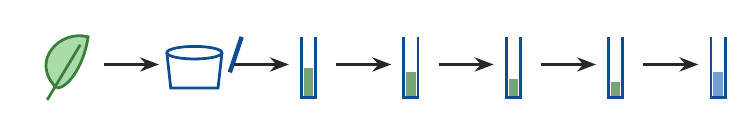
\begin{tikzpicture}[line width=1pt]
  % hoja
  \begin{scope}[shift={(0,0)}]
    \draw[apVerde, fill=apVerdeClaro] (0,-0.3) .. controls (-0.35,0.05) and (0.05,0.45) .. (0.4,0.35) .. controls (0.35,0.0) and (0.15,-0.3) .. (0,-0.3);
    \draw[apVerde] (-0.12,-0.45) -- (0.3,0.25);
  \end{scope}
  \draw[->, apNegro] (0.6,0) -- (1.3,0);
  % vaso con varilla
  \begin{scope}[shift={(1.75,-0.05)}, apAzul]
    \draw (-0.35,0.2) -- (-0.3,-0.25) -- (0.3,-0.25) -- (0.35,0.2);
    \draw (0,0.2) ellipse (0.35 and 0.08);
    \draw[line width=1.6pt] (0.45,-0.05) -- (0.6,0.4);
  \end{scope}
  % tubos: cada vez menos material (verde) y más claro
  \foreach \i/\x/\col/\alto in {1/3.2/apVerde/0.35, 2/4.5/apVerde/0.3, 3/5.8/apVerde/0.22, 4/7.1/apVerde/0.18, 5/8.4/apAzulClaro/0.3} {
    \draw[->, apNegro] ({\x-0.95},0) -- ({\x-0.25},0);
    \fill[\col!70] ({\x-0.06},-0.4) rectangle ({\x+0.06},{-0.4+\alto});
    \draw[apAzul] ({\x-0.09},0.35) -- ({\x-0.09},-0.42) -- ({\x+0.09},-0.42) -- ({\x+0.09},0.35);
  }
\end{tikzpicture}
% ---------------------------
\end{document}
